
\begin{quote}
Code sollte gut verständlich und wartbar sein. Dazu gehört, dass Dateien und Funktionen nicht zu komplex sind. Sehr komplexer Code ist schwer zu verstehen, zu testen und zu warten. Komplexität lässt sich durch verschiedene Metriken messen, z.B. durch die zyklomatische Komplexität, die die Anzahl möglicher Pfade durch eine Funktion angibt. Ab etwa 50 Pfaden wird Code schwer verständlich, ab 100 Pfaden sehr schwer.

In der Analyse wurden viele unnötig komplexe Funktionen verteilt über die gesamte Software gefunden: sehr lange Methoden, stark verschachtelte Strukturen, fehlende Guard-Clauses und kaum Hilfsfunktionen. Moderne Sprachfeatures wie Switch(-Expressions) oder Pattern Matching werden selten genutzt, sodass Logik oft unstrukturiert in großen Funktionen zusammengefasst ist. Dies zeigt sich deutlich an der hohen zyklomatischen Komplexität einiger Dateien. Manche wenige Dateien sind sogar extrem komplex (über 200).

Zu erkennen an den roten Gebäuden, verteilt über das gesamte Bild.

Wir empfehlen, besonders die sehr komplexen und großen Dateien zu überarbeiten und zu vereinfachen.

Legende:  
Fläche = Anzahl der Codezeilen (höchster Wert: 2785)  
Höhe = Anzahl der Autoren (höchster Wert: 20)  
Farbe = Zyklomatische Komplexität (1-524, 10=grün, 200=rot)
\end{quote}

\begin{figure}[H]
    \centering
    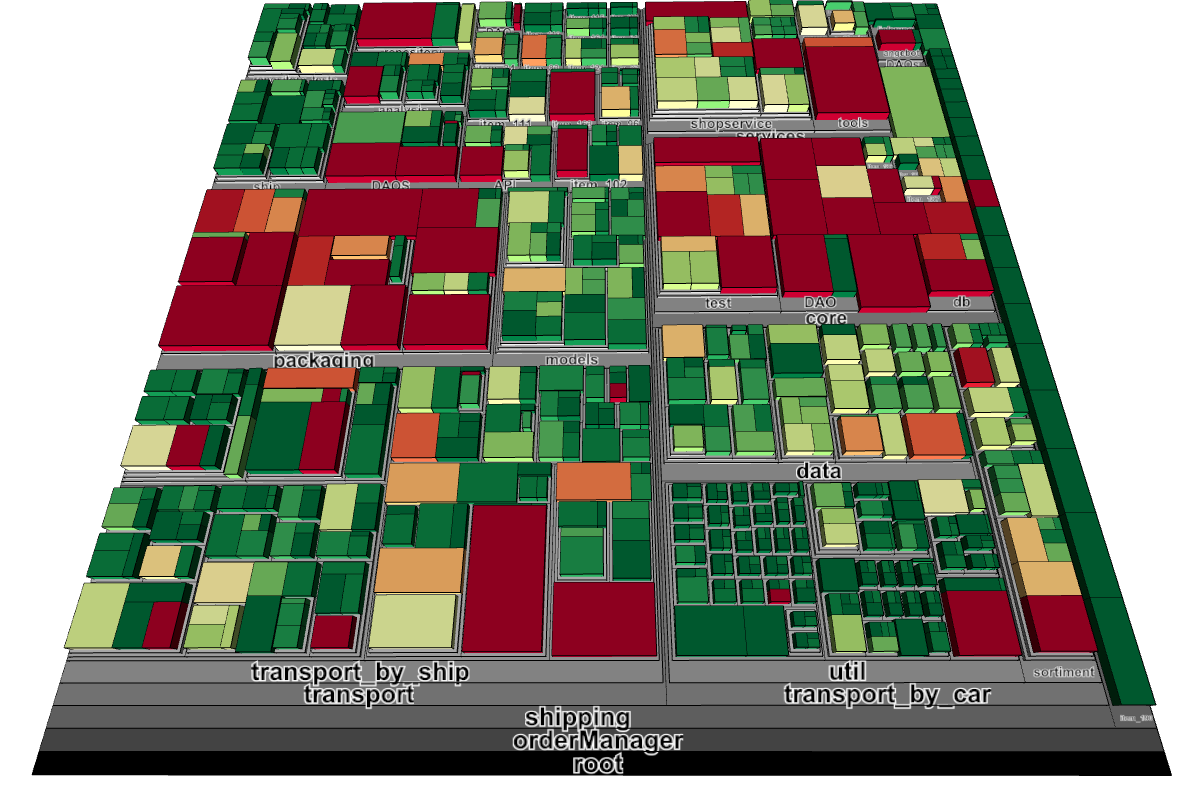
\includegraphics[width=0.8\textwidth]{images/umfrage/treemap/komplex.png}
    \caption[Bild aus Szenario: Hohe Komplexität]{Bild aus Szenario: Hohe Komplexität in einzelnen Funktionen, Fläche: Anzahl der Codezeilen, Höhe: Anzahl der Autoren, Farbe: Zyklomatische Komplexität}
\end{figure}

\begin{quote}
    Wie sehr hilft dir die Visualisierung, die Analyse der Experten nachzuvollziehen?
\end{quote}